% Credits are indicated where needed. The general idea is based on a template by Vel (vel@LaTeXTemplates.com) and Frits Wenneker.

\documentclass[11pt, a4paper]{article} % General settings in the beginning (defines the document class of your paper)
% 11pt = is the font size
% A4 is the paper size
% “article” is your document class

%----------------------------------------------------------------------------------------
%	Packages
%----------------------------------------------------------------------------------------

% Necessary
\usepackage[german,english]{babel} % English and German language 
\usepackage{booktabs} % Horizontal rules in tables 
% For generating tables, use “LaTeX” online generator (https://www.tablesgenerator.com)
\usepackage{comment} % Necessary to comment several paragraphs at once
\usepackage[utf8]{inputenc} % Required for international characters
\usepackage[T1]{fontenc} % Required for output font encoding for international characters

% Might be helpful
\usepackage{amsmath,amsfonts,amsthm} % Math packages which might be useful for equations
\usepackage{tikz} % For tikz figures (to draw arrow diagrams, see a guide how to use them)
\usepackage{tikz-cd}
\usetikzlibrary{positioning,arrows} % Adding libraries for arrows
\usetikzlibrary{decorations.pathreplacing} % Adding libraries for decorations and paths
\usepackage{tikzsymbols} % For amazing symbols ;) https://mirror.hmc.edu/ctan/graphics/pgf/contrib/tikzsymbols/tikzsymbols.pdf 
\usepackage{blindtext} % To add some blind text in your paper
\usepackage{hyperref}


%---------------------------------------------------------------------------------
% Additional settings
%---------------------------------------------------------------------------------

%---------------------------------------------------------------------------------
% Define your margins
\usepackage{geometry} % Necessary package for defining margins

\geometry{
	top=2cm, % Defines top margin
	bottom=2cm, % Defines bottom margin
	left=2.2cm, % Defines left margin
	right=2.2cm, % Defines right margin
	includehead, % Includes space for a header
	%includefoot, % Includes space for a footer
	%showframe, % Uncomment if you want to show how it looks on the page 
}

\setlength{\parindent}{15pt} % Adjust to set you indent globally 

%---------------------------------------------------------------------------------
% Define your spacing
\usepackage{setspace} % Required for spacing
% Two options:
\linespread{1.5}
%\onehalfspacing % one-half-spacing linespread

%----------------------------------------------------------------------------------------
% Define your fonts
\usepackage[T1]{fontenc} % Output font encoding for international characters
\usepackage[utf8]{inputenc} % Required for inputting international characters

\usepackage{XCharter} % Use the XCharter font


%---------------------------------------------------------------------------------
% Define your headers and footers

\usepackage{fancyhdr} % Package is needed to define header and footer
\pagestyle{fancy} % Allows you to customize the headers and footers

%\renewcommand{\sectionmark}[1]{\markboth{#1}{}} % Removes the section number from the header when \leftmark is used

% Headers
\lhead{} % Define left header
\chead{\textit{}} % Define center header - e.g. add your paper title
\rhead{} % Define right header

% Footers
\lfoot{} % Define left footer
\cfoot{\footnotesize \thepage} % Define center footer
\rfoot{ } % Define right footer


%---------------------------------------------------------------------------------
%	General information
%---------------------------------------------------------------------------------
\title{Restaurant diversity in Boston neighborhods} % Adds your title
\author{
Brian Schaefer % Add your first and last name
    %\thanks{} % Adds a footnote to your title
    %\institution{YOUR INSTITUTION} % Adds your institution
  }

\date{\small \today} % Adds the current date to your “cover” page; leave empty if you do not want to add a date


%---------------------------------------------------------------------------------
%	Define what’s in your document
%---------------------------------------------------------------------------------

\begin{document}


% If you want a cover page, uncomment "\input{coverpage.tex}" and uncomment "\begin{comment}" and "\end{comment}" to comment the following lines
%\input{coverpage.tex}

%\begin{comment}
\maketitle % Print your title, author name and date; comment if you want a cover page 

%\end{comment}

%----------------------------------------------------------------------------------------
% Introduction
%----------------------------------------------------------------------------------------
\setcounter{page}{1} % Sets counter of page to 1

\section{Introduction}

Residents and frequent visitors of Boston are certainly familiar with its famous cultural centers and the food options each one provides.
Popular neighborhoods including Chinatown, North End, and the Seaport District are hot spots for those looking to indulge in the city's best Chinese, Italian, and seafood options.
But, where should one go for a more diverse selection of restaurants?
In this study, we classify neighborhoods in Boston based on restaurant variety and identify the neighborhoods with the most diverse options.

\section{Data}

To classify Boston's neighborhoods, we need geographical information about the neighborhoods as well as information on the types of restaurants that exist within each neighborhood.
For the former, we use geographical coordinates provided by the City of Boston outlining the boundaries of each of Boston's neighborhoods\footnote{\url{https://data.boston.gov/dataset/boston-neighborhoods}}.
For the latter, we use Foursquare\footnote{\url{https://www.foursquare.com}} to gather information on the types of restaurants nearby the geographical center of each neighborhood.

The geographical data are provided in \texttt{GeoJSON} format.
The dataset consists of multiple sets of \texttt{(longitude, latitude)} coordinates that define the boundaries of each neighborhood.
We adapt functions from the \texttt{geojson\_utils} Python package\footnote{\url{https://pypi.org/project/geojson_utils/}} to calculate the coordinates of the centroid and area of each neighborhood given the list of boundary coordinates.
Using the Python package \texttt{folium}, we can show the neighborhoods on an interactive map (Figure 1).

\begin{figure}
\begin{center}
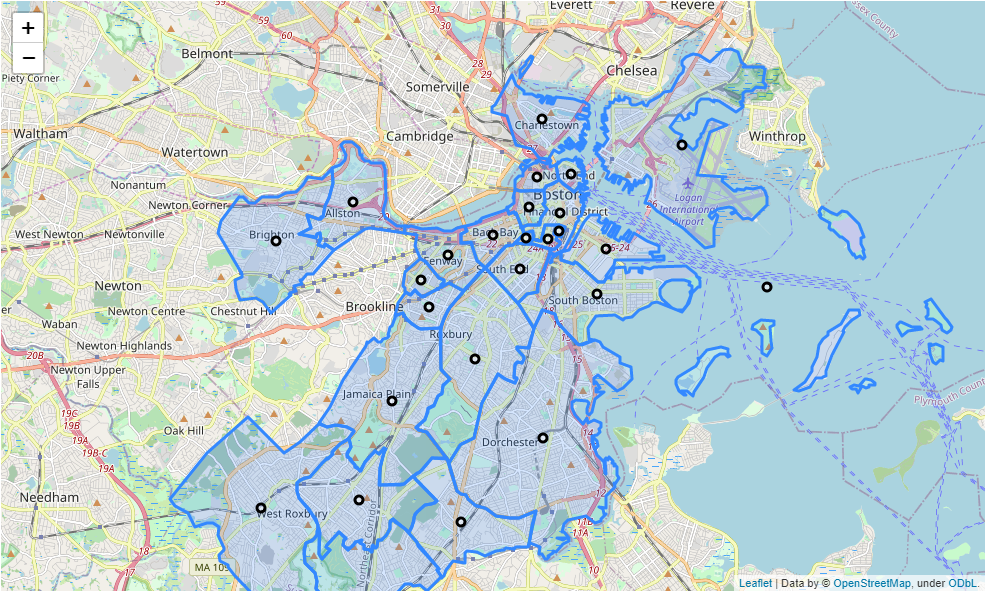
\includegraphics[width=0.7\textwidth]{folium_map.png}
\end{center}
\caption{Map of Boston neighborhoods (blue) and geographical centers (black markers).}
\end{figure}

We use the Foursquare application programming interface (API) to search for restaurants nearby each neighborhood's geographical center using the category ``Food''\footnote{\texttt{categoryId 4d4b7105d754a06374d81259}, \url{https://developer.foursquare.com/docs/build-with-foursquare/categories/}.}.
The Foursquare service returns the venue name, geographical coordinates, address, and category name for each of the ``Food'' venues found in the vicinity of each search point.
Since we are interested in unique types of restaurants in each neighborhood, we take the category name for each venue and ignore venues in the same neighborhood with the same name.
Figure 2 shows a summary of the relative frequencies of different types of venues across all neighborhoods. 
There are a few venue types that occur with very high frequency, and a relatively large number of unique venue types.

\begin{figure}
\begin{center}
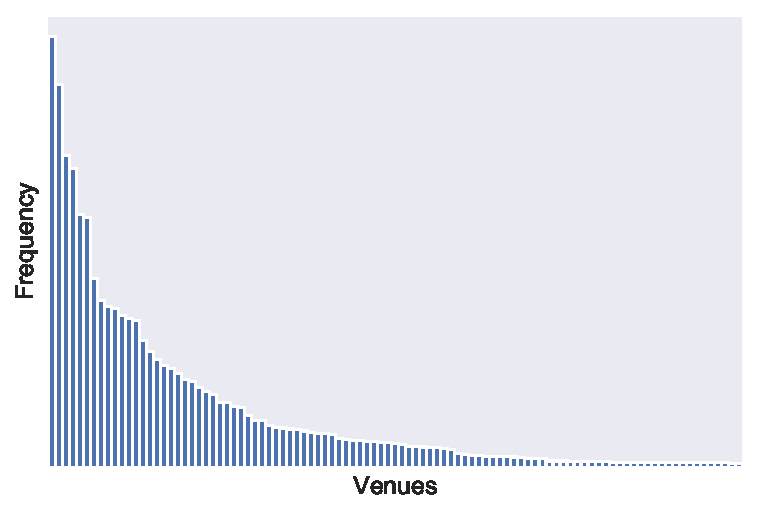
\includegraphics[width=0.7\textwidth]{summary_bar.pdf}
\end{center}
\caption{Frequency of venue types across all Boston neighborhoods.}
\end{figure}





%---------------------------------------------------------------------------------

\end{document}